Neste capítulo será apresentado em detalhes as premissas do problema de classificação visual bem como a metodologia para sua solução, que será particionada nas conforme proposto a seguir. A seção~\ref{sec:Cap3_Dataset} apresenta o conjunto de dados utilizado para o experimento.  A seção~\ref{sec:Cap3_Premissas} apresenta as limitações e condições de contorno do problema. A seção~\ref{sec:Cap3_Proposta} apresenta a proposta de solução para o problema. A seção~\ref{sec:Cap3_Procedimentos} apresenta os procedimentos do experimento para treino e teste do modelo. Dessa forma, a metodologia será seccionada nas seguintes partes:

\begin{itemize}
    \item  Datasets.
    \item  Premissas do problema.
    \item  Proposta de solução.
    \item  Experimento para a solução do problema.

\end{itemize}

% ----------------------------------------------------------

\section{\textit{Conjunto de dados}}\label{sec:Cap3_Dataset}
Foram utilizados dois conjuntos de dados, escolhidos por razões de disponibilidade e representatividade do problema. 

%% Tabelas dos datasets
%- Million A1
%ASGM Ponds Dataset https://zenodo.org/record/6400211
% Planet (URL: https://www.kaggle.com/c/planet-understanding-the-amazon-from-space/data

\subsection{Dataset amazônia do espaço}\label{sec:Cap3_Amazon_dataset}

Este dataset foi publicado em uma competição Kaggle, pela empresa Planet\footnote{https://www.kaggle.com/c/planet-understanding-the-amazon-from-space/data}. Possui resolução de $3 m$ de píxel. Dados foram coletados dos satélites Planet Flock entre 2016 e 2017. Todas as imagens são da bacia amazônica. Este dataset concerne ao desmatamento de mangues. Cada amostra é um recorde de $256 \times 256$ pixeis RGB, pertencente a 14 classes distintas. Cobrindo condições atmosféricas, coberturas de terreno e fenômenos raros. Foi utilizado em ~\cite{9701667} citado no capitulo anterior.

\begin{figure}[!ht]
    \centering
    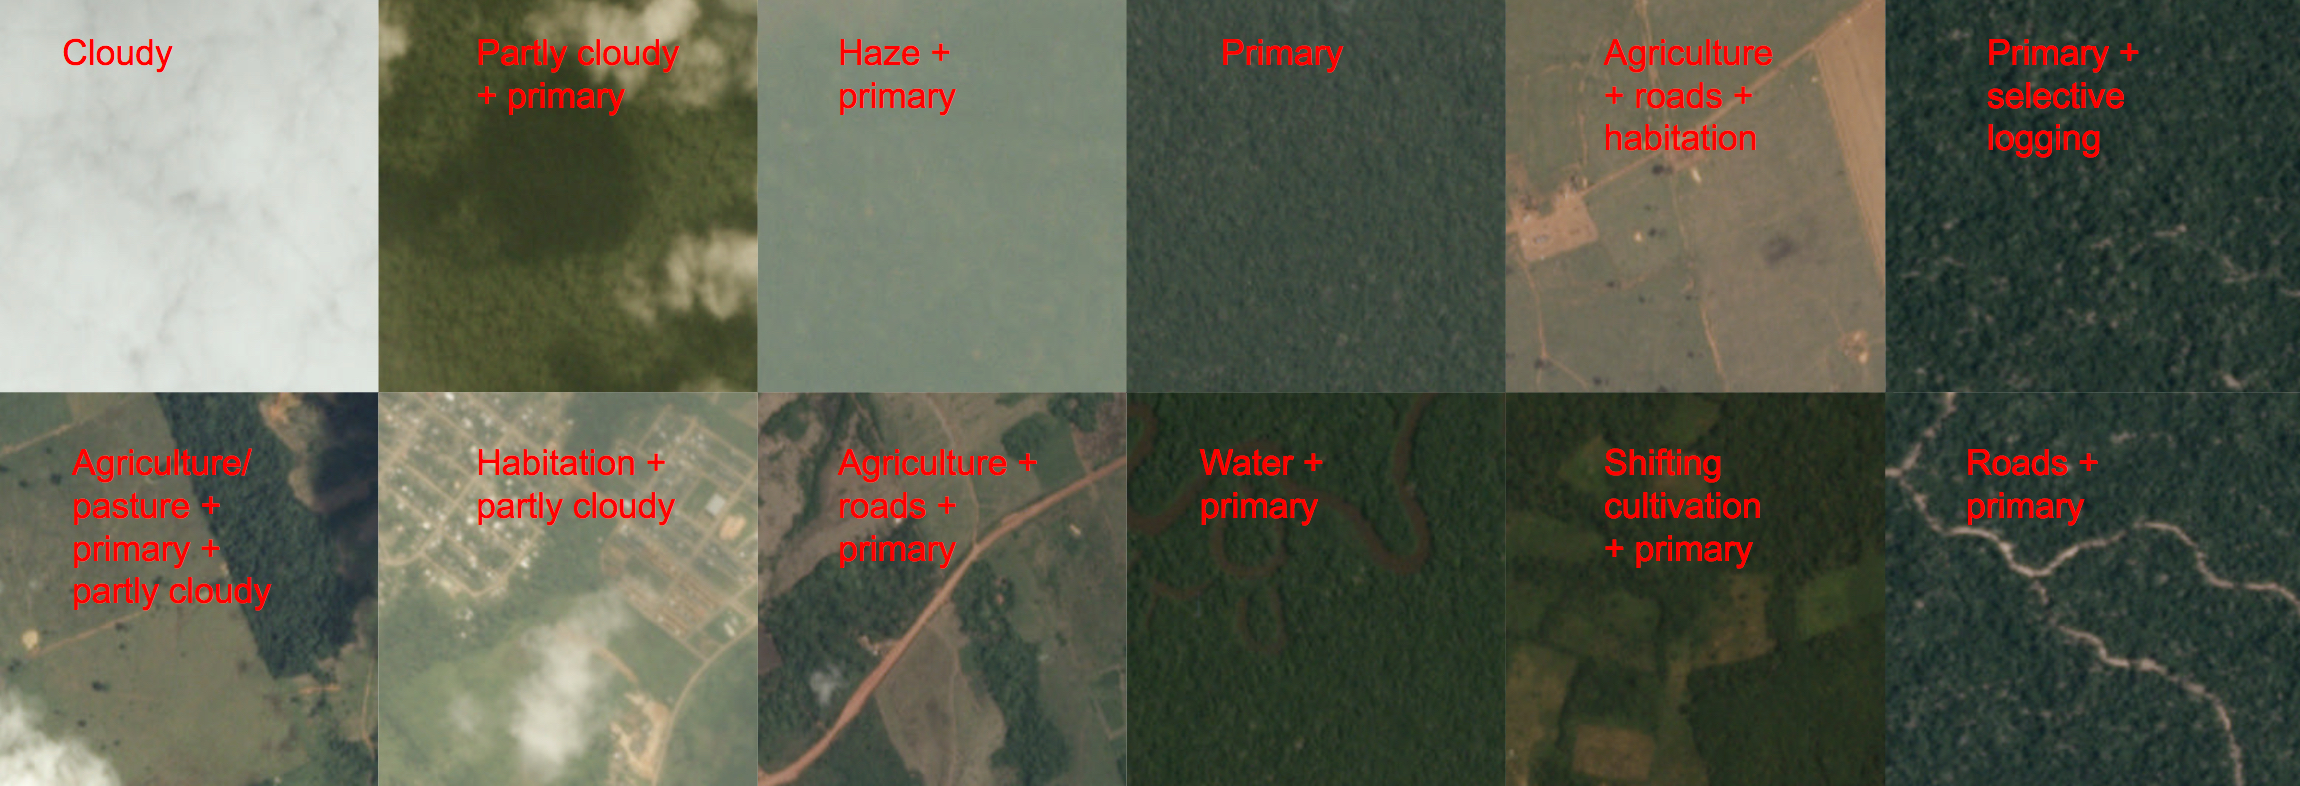
\includegraphics[width=0.9\columnwidth]{
        Imagens/chips.jpg
    }
    \caption{Amostras de classes do dataset Amazônia do espaço}\label{fig:dataset}
\end{figure}

%We utilize a dataset (URL: https://www.kaggle.com/c/planet-understanding-the-amazon-from-space/data) published in a Kaggle competition (by Planet company), containing coarse-resolution imagery data from satellites with varying spatial resolution characteristics, i.e., the imagery has a ground-sample distance (GSD) of 3.7 m and an orthorectified píxel size of 3 m. The data comes from Planet’s Flock tow satellites in both Sun-synchronous and ISS orbits and was collected in the time interval between January 1, 2016, and February 1, 2017. All of the images are derived from the Amazon basin. Mangrove deforestation in the Amazon forest is an intense phenomenon, and a plethora of factors that contribute to deforestation is observed there. Each entry contains imagery data in RGB plus the infrared band in geo-referenced.tiff format. In our experiment, the images are classified into 14 classes and the labels are broken into three groups: atmospheric conditions, common land cover/land use phenomena, and rare land cover/land use phenomena (see Fig. 3). Here, each entry is assigned to one or more classes.


\subsection{Dataset poças de garimpo}\label{sec:Cap2_amazonia_garimpo}

Este \textit{dataset} foi utilizado em \cite{rs14071746}, mencionado no capitulo anterior. Concerne a tarefa de identificação de mudanças de imagem. Aplicadas a identificação de garimpo artesanal de ouro de pequena escala; Pode ser desafiador de se identificar, dado a variabilidade de condições atmosféricas e baixa resolução. Foram utilizadas imagens de Madre de Dios, região do Peru. Bem como amostras de outros países: Venezuela, Indonésia e Myanmar. 

% (Verificar se esse dataset é utilizável para tarefa de classificação; Resolução parece muito baixa e área muito grande)

% Abstract: Monitoring changes within the land surface and open water bodies is critical for natural resource management, conservation, and environmental policy. While the use of satellite imagery for these purposes is common, fine-scale change detection can be a technical challenge. Difficulties arise from variable atmospheric conditions and the problem of assigning píxels to individual objects. We examined the degree to which two machine learning approaches can better characterize change detection in the context of a current conservation challenge, artisanal small-scale gold mining (ASGM). We obtained Sentinel-2 imagery and consulted with domain experts to construct an open-source labeled land-cover change dataset. The focus of this dataset is the Madre de Dios (MDD) region in Peru, a hotspot of ASGM activity. We also generated datasets of active ASGM areas in other countries (Venezuela, Indonesia, and Myanmar) for out-of-sample testing.


% Dataset Description

%- Understanding the Amazon from Space [20] — multilabel dataset to track the human footprint in the Amazon rainforest; we’ll mostly refer to this as the Amazon dataset.
%WiDS Datathon 2019 [21] — binary dataset for oil palm plantation detection in Borneo; we’ll mostly refer to this as the oil palm dataset.
% Towards Detecting Deforestation [22] — binary dataset for detecting coffee plantations in the Amazon rainforest; we’ll mostly refer to this as the coffee dataset.


% ----------------------------------------------------------

\section{\textit{Premissas}}\label{sec:Cap3_Premissas}

Temos que o problema de identificação em sensoriamento remoto impõe a dificuldade de alta similaridade extra-classes e divergências intra-classes, da qual surge uma dificuldade de generalização e de viés indutivo para identificação de amostras fora das classes treinadas. Temos ainda que o treinamento de tais modelos envolvem um volume massivo de amostras e de custo computacional. 


% ----------------------------------------------------------

\section{\textit{Proposta de solução}}\label{sec:Cap3_Proposta}

Como solução para o problema, foi proposta a utilização de um modelo ViT pré-treinado com um dataset expressivo e realizar o fine-tune para o conjunto de dados de interesse. Dessa forma, obtendo um modelo com boa capacidade de generalização e com menor custo computacional para ser treinado.

Para solucionar o problema de generalização e dataset limitado da região de interesse, propomos a utilização de um modelo pré-treinado explicado em~\ref{sec:Cap2_transfer} um dataset extensivo de imagens aéreas e de satélites, de forma a aproveitar seu extrator de características, como é realizado em~\cite{wang2022empirical}. Assim o modelo será re-treinado (\textit{fine tunning}) para a região de interesse mantendo os pesos das camadas de encoder otimizar apenas a camada MLP fortemente conectadas, assim como a camadas de saídas softmax. 

Dessa forma, a arquitetura proposta é o ViT apresentado em~\cite{wang2022empirical}
composta por camadas hierarquicas de encoders transformers  que funcionam como extratores de características. As camadas seguintes são camadas totalmente conectadas seguidas por uma camada \textit{softmax} que realiza a classificação.
% ----------------------------------------------------------

\section{\textit{Ambiente e ferramentas}}\label{sec:Cap3_Ferramentas}


O Ambiente dos experimentos será em cadernos \textit{Jupyters}, para ser facilmente replicável e ser executável em nuvem, com a possibilidade de alugar recursos computacionais da plataforma em nuvem \textit{Google Collab}. Também será utilizado o \textit{framework PyTorch}, por razões de disponibilidade de métodos e conhecimentos do autor.

\subsection{\textit{PyTorch}}\label{sec:Cap2_PyTorch}
Pytorch é um \textit{framework}\footnote{Ferramental} código aberto de Python para aprendizado de máquinas. É implementado em linguagens C++ e CUDA para otimizações de computações numéricas e matriciais, que são extensivas para esta aplicação.
Foi desenvolvido pelo Facebook e é atualmente amplamente adotado pela comunidade de pesquisa e mercado de aprendizado de máquina. Possui muitas implementações das ferramentas mais utilizadas, especificamente aplicadas a \textit{Deep Learning} e visão computacional. Tem ampla adoção devido à intenção de ser um \textit{framework} de fácil uso e alto nível, com muitas abstrações e técnicas já implementadas.


% ----------------------------------------------------------


% TODO: citar o paper de aplicação direta
\section{\textit{Experimentos}}\label{sec:Cap3_Experimentos}

Para a construção da nossa solução desejada, experimentaremos combinar um modelo pré-treinado com camadas internas e de saída treinadas para a região de interesse.
Consiste em fazer experimentos em uma complexidade crescente, e replicando resultados para garantir corretude. Será simplificado a reprodução para apenas um \textit{dataset}.


Para obter o modelo proposto e de melhor desempenho, foi proposto a seguinte sequência de experimentos para construir o modelo final:

\begin{enumerate}
\item  Replicar experimentos dos trabalhos~\ref{sec:Cap2_million} com \textit{checkpoints}\footnote{Captura dos pesos de uma rede a partir de certo ponto do processo de treino} disponibilizados. 
\item  Replicar experimentos de \ref{sec:Cap2_ForestViT} em um modelo base de comparação baseado em em uma CNN ResNet-50
\item  Replicar o experimento do~\ref{sec:Cap2_ForestViT} utilizando um modelo ViT pré treinado para sensoriamento remoto
\item Avaliar desempenho, comparar com os experimentos e trabalhos bases \ref{sec:Cap2_revisao_literatura}
\end{enumerate}


    
% ----------------------------------------------------------

\section{\textit{Procedimentos}}\label{sec:Cap3_Procedimentos}

Os procedimentos do experimento principal consiste principalmente nas etapas de 
pré-processamento, treino e validação. Explicadas adiante.

\subsection{\textit{Pré-processamento}}\label{sec:Cap3_PreProcess}
O pré-processamento consistem em preparar as amostras do conjunto de dados de interesse para treino e validação. Para o conjunto de dados floresta amazônica temos 40000 amostras de treino e 4000 de teste. Cada recorte de resolução $256 \times 256$ px é aplicado um \textit{downsampling}\footnote{Subamostragem} para a resolução de entrada do modelo pré-treinado, de $224 \times 224$. 

\subsection{\textit{Treino}}\label{sec:Cap3_Treino}
Para a etapa de treino, utilizamos a arquitetura proposta em~\ref{sec:Cap3_Proposta}, que consiste em um modelo pré-treinado, e retreinando suas ultimas camadas de classificação por camadas fortemente conectadas seguidas de camadas de \textit{softmax}, como ilustra a imagem a seguir:


% TODO Imagem da arquitetura proposta.



\subsection{\textit{Validação}}\label{sec:Cap3_Validacao}

A etapa de validação será realizada a medida do desempenho do modelo no conjunto de testes para classificação.



% 5. Experiments
%  - [ ] Steps
%  - [ ] Resume
 % - [ ] Baseline
 % - [ ] Pipeline
